% Created 2019-10-31 jeu. 11:10
% Intended LaTeX compiler: pdflatex
\documentclass[a4paper, keeplastbox, biblatex]{jacow}
\usepackage[utf8]{inputenc}
\usepackage[T1]{fontenc}
\usepackage{graphicx}
\usepackage{grffile}
\usepackage{longtable}
\usepackage{wrapfig}
\usepackage{rotating}
\usepackage[normalem]{ulem}
\usepackage{amsmath}
\usepackage{textcomp}
\usepackage{amssymb}
\usepackage{capt-of}
\usepackage{hyperref}
\usepackage[most]{tcolorbox}
\usepackage{siunitx}
\usepackage{pdfpages,multirow,ragged2e}
\usepackage{graphicx,tabularx,booktabs}
\usepackage{blindtext}
\usepackage[USenglish, english]{babel}
\addbibresource{ref.bib}
\setcounter{footnote}{1}
\author{T. Dehaeze\textsuperscript{1,}\thanks{thomas.dehaeze@esrf.fr}, M. Magnin-Mattenet, ESRF, Grenoble, France \\ C. Collette\textsuperscript{1}, Université Libre de Bruxelles, BEAMS department, Brussels, Belgium \\ \textsuperscript{1}also at Precision Mechatronics Laboratory / A\&M department, Liege, Belgium}
\date{2019-10-31}
\title{SAMPLE STABILIZATION FOR TOMOGRAPHY EXPERIMENTS IN PRESENCE OF LARGE PLANT UNCERTAINTY}
\begin{document}

\maketitle

\begin{abstract}
A new low emittance lattice storage ring is under construction at the ESRF.
In this new instrument, an upgraded end station for ID31 beamline must allow to position the samples along complex trajectories with a nanometer precision.
In order to reach these requirements, samples have to be mounted on high precision stages, combining a capability of large stroke, spin motion, and active rejection of disturbances.
First, the end station will be presented with the associated requirements. However, the precision is limited by thermal expansion and various imperfections that are not actively compensated.
Our approach is to add a Nano Active Stabilization System (NASS) which is composed of a 6DoF Stewart platform and a 6 DoF metrology system.
A 3D model of the end station updated with experimental data is developed.
As the mass of the samples may vary by up to two orders of magnitudes, robust control strategies are required to address such plant uncertainty.
The proposed control strategy are presented and applied on the developed model by conducting time domain simulations of tomography experiment in presence of instrumentation noise and system uncertainty.
\end{abstract}

\section{INTRODUCTION}
\label{sec:orgdf25a9c}
Within the framework of the ESRF Phase II Upgrade Programme, a new state-of-the-art end station for the high-energy beamline ID31 is under development.
Research in many scientific areas such as material and life sciences are increasingly looking for instruments with higher spatial resolution.
The design of the new end station will enable many hard X-ray characterization techniques such as reflectivity, wide angle diffraction and diffraction tomography.
The need of great versatility induces many constrains on the end station such as combining large stroke (\(\approx\SI{10}{\milli\metre}\)), high precision (\(\approx\SI{10}{\nano\metre}\)) while accepting samples with mass ranging from \(\SI{1}{\kilo\gram}\) to \(\SI{50}{\kilo\gram}\).

Many positioning end stations have been developed with an increasing positioning precision \cite{martinez2016,DucotteMEDSI2016,ogurreck2013nanotomography}.

However, when nanometer precision is needed, thermal expansion and vibrations are becoming the main source of positioning error that cannot be compensated by encoders used for each stage.
Therefore, a direct metrology system is usually needed \cite{DucotteMEDSI2016}.

The aim of this study is to develop a short stroke Stewart platform that actively stabilize the sample position and compensate for all sources of perturbations and imperfection.

This paper is organized as follows into three sections.
The first section presents the ID31 positioning end station and its associated specifications.
The second section is dedicated to the Nano Active Stabilization System (NASS) and the associated metrology frame. A model of the ID31 positioning station is also developed and presented.
In the third section, after presenting the control strategy, simulations of tomography experiments are conducted using the developed model. These measurements are used to estimate the performance gain of using such active stabilization system.

\section{ID31 SAMPLE-STATION}
\label{sec:orgaeecefa}
In order to position the samples along complex trajectories with a nanometer precision, a versatile positioning platform is developed. A simplified schematic representation of the system is shown Fig. \ref{fig:schematic_sys_without_nass}.

\subsection{Design}
\label{sec:org6bd25e8}
\begin{figure}[htbp]
\centering
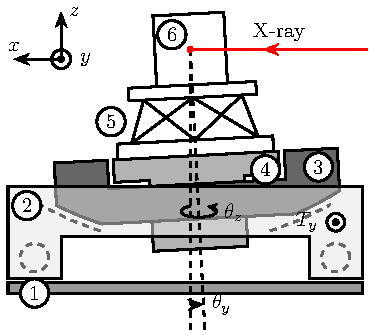
\includegraphics[scale=1]{./figs/schematic_sys_without_nass.pdf}
\caption{\label{fig:schematic_sys_without_nass}
Schematic representation of the ID31 end station. (1) granite, (2) Translation Stage, (3) Tilt Stage, (4) Spindle, (5) Long Stroke Hexapod, (6) Sample.}
\end{figure}

\begin{figure*}
\centering
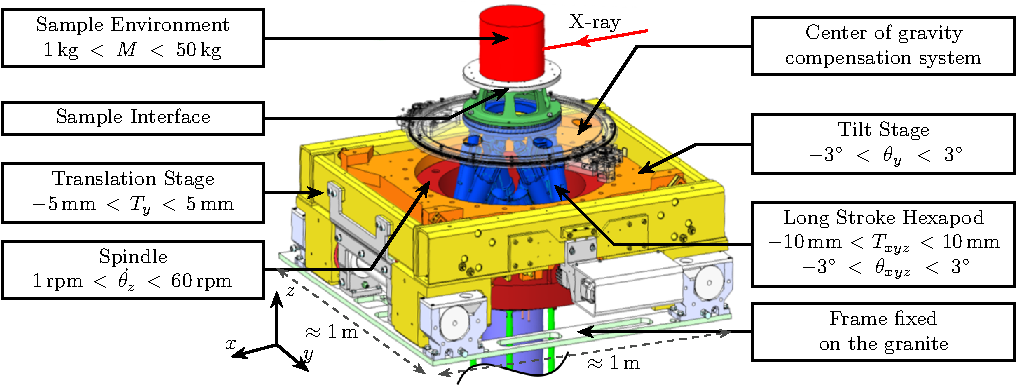
\includegraphics[scale=1]{./figs/assemblage.pdf}
\caption{\label{fig:assemblage}
CAD view of the ID31 end station.}
\end{figure*}

This platform consists of multiple stacked stages, each of which is described below.

First, a translation stage offers a travel range of \(T_y = \SI{\pm5}{\milli\metre}\) in the \(y\) direction which permits to scan the sample through the X-ray.
A linear encoder is used to drive a brush-less linear motor in a feedback loop with a Proportional-Integral-Derivative (PID) control law.

A tilt stage then rotates the sample around the \(y\) axis by \(\theta_y = \ang{\pm3}\). The rotation axis is aligned with the focusing point of the X-ray in order to allow experiments such as X-ray reflectivity.
The tilt stage is driven by a stepper motor and a PI position feedback using linear encoders.

An air bearing spindle permits to rotate the sample around the vertical axis with an angular speed that varies from \(\dot{\theta_z} = \SI{1}{rpm}\) for light samples (\(M<\SI{1}{\kilo\gram}\)) to \(\dot{\theta_z} = \SI{60}{rpm}\) for heavy samples (\(M=\SI{50}{\kilo\gram}\)).

A long-stroke Stewart platform developed by Symetrie is placed on top of the spindle. It allows a fine positioning of the sample in all 6 degrees of freedom (DoF). Each leg of the Hexapod has an absolute linear encoder and a DC motor.

As the center of mass of the stages above the spindle is not perfectly aligned with the spindle axis, centrifugal forces generate parasitic motions.
To overcome this issue, a center of gravity compensation system is used (Fig. \ref{fig:assemblage}). It consists of two motorized mass that can be positioned around a circular guidance in order to perfectly aligned the center of mass with the spindle rotation axis.

Finally a sample environment is positioned on top of all the stages. The sample environment permits to study samples under wide range of condition: low (\(\SI{1.2}{\kelvin}\)) to high (\(\SI{2000}{\kelvin}\)) temperatures, high magnetic field (\(\SI{8}{\tesla}\)), etc.

A CAD view of the platform is shown Fig. \ref{fig:assemblage}. The green mechanical element shown below the sample environment is a rigid element that support the sample interface. It will later be replaced by the NASS.

\subsection{Specifications}
\label{sec:org050f06e}
As shown in the previous section, the positioning system is composed of numerous stages in order to allow complex trajectories for various experiments.

As the precision needed on the sample position is very depending of the experiment conducted, only the most stringent requirements are summarized on Table \ref{table:specifications}.
Moreover the metrology system must remain stable for 8 hours within \(\SI{10}{\nano\metre}\).

\begin{table}[!htpb]
\caption{\label{table:specifications}
Summary of the most stringent specifications on the motions of the ID31 end station}
\centering
\begin{tabular}{ccccc}
\hline
 & \(T_{xy}\) & \(T_z\) & \(\theta_y\) & \(\theta_z\)\\
\hline
Repeatability & \(\SI{20}{\nano\metre}\) & \(\SI{10}{\nano\metre}\) & \(\SI{5}{\micro\radian}\) & \(\SI{2}{\micro\radian}\)\\
\hline
MIM\footnotemark & \(\SI{3}{\nano\metre}\) & \(\SI{3}{\nano\metre}\) & \(\SI{2}{\micro\radian}\) & \(\SI{0.5}{\micro\radian}\)\\
\hline
\end{tabular}
\end{table}

\footnotetext{Minimum Incremental Motion}

As the experiment with the most stringent requirements is the diffraction tomography, it will be used for simulations in order to test the performances of the system.

\subsection{Measurements On The Existing End Station}
\label{sec:org55d0f26}
Measurements have been conducted on each stage separately in order to characterize their positioning precision and mechanical properties.

Moreover, measurements have been done on the mounted end station (Fig. \ref{fig:exp_setup}) to identify its mechanical behavior.
These measurements will permit to tune the parameters of the developed model to better match the physical system.

\begin{figure}[htbp]
\centering
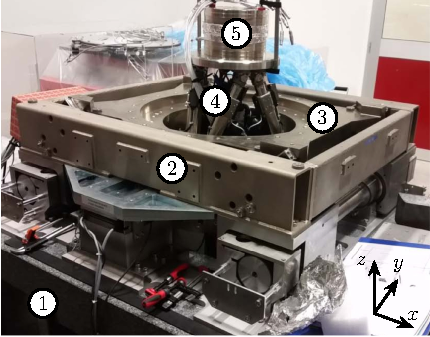
\includegraphics[scale=1,width=0.95\linewidth]{./figs/exp_setup.pdf}
\caption{\label{fig:exp_setup}
Picture of the ID31 end station. (1) Granite, (2) Translation stage, (3) Tilt stage, (4) Long stroke hexapod, (5) Mass representing the sample environment. The spindle is hidden by the translation and tilt stages.}
\end{figure}

\section{NANO ACTIVE STABILIZATION SYSTEM}
\label{sec:org7cadf36}
\subsection{6 DoF Metrology System}
\label{sec:org16eceaa}
Even though the precision of each stage has shown to be excellent, thermal drifts and various parasitic motions cannot be compensated by the encoders used.
Moreover, we want to control the position of the sample with respect to the X-ray that is determined by the position of the optical elements.

In order to achieve the positioning accuracy and stability requirements (shown on Table \ref{table:specifications}), a direct measurement of the relative position from the sample to the optical element is mandatory.
Laser interferometry is chosen as it offers many advantages such as high resolution, high stability and large measurement range.

A 6 DoF metrology system is still under developed. Therefore, this is not developed in this paper.

\subsection{6 DoF Active Stabilization Stage}
\label{sec:orge67f457}
In order to actively compensate the positioning error of the sample in all 6 DoF, a short stroke Stewart platform (the NASS) is added between the long stroke hexapod and the sample (Fig. \ref{fig:system_control}).

A Stewart platform is a parallel robot that consists of two platforms connected by 6 active legs. Each leg has one actuator and two rotational joints \cite{McInroy1999a}. The actuators can either be piezo electric stacks or voice coil linear actuators.

By inverting the dynamics of the Stewart platform, it is possible to control independently the position of the mobile platform in all 6 DoF with respect to the fixed platform \cite{McInroy2000}.

These Stewart platforms have been extensively used for vibration control \cite{Geng1992,preumont2007} as it offers many advantages over conventional stacked stages such as high stiffness and high load over weight ratio.

\subsection{Control Objective}
\label{sec:orgf7bd3ce}
The control objective is to stabilize the position of the sample using the NASS actuators based on the 6DoF measurements provided by the metrology system.

By this way, all the imperfections that are presently corrected (thermal drifts, guidance flexibilities, etc.) will be measured and compensated using a feedback control loop.

Figure \ref{fig:system_control} shows a simplified control architecture which will be used for the NASS. The validation and optimization of this control is done on a separate test bench.

\begin{figure}[htbp]
\centering
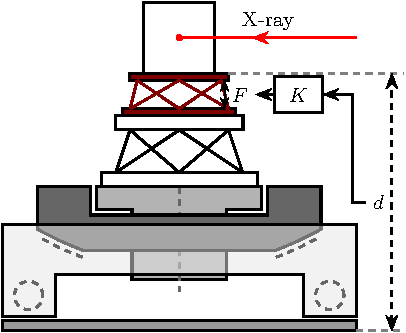
\includegraphics[scale=1]{./figs/system_control.pdf}
\caption{\label{fig:system_control}
Schematic representation of the NASS added below the sample and the control architecture used.}
\end{figure}

\subsection{Requirements For The NASS}
\label{sec:org24c8374}
The required stroke for the NASS should correspond to the maximum global positioning error of the end station without the NASS.
This has been estimated to be around \(\SI{10}{\micro\metre}\) in translations. This value will be confirmed as soon as full tests of the micro-station will be finalized.

Then, the minimum repetability of the NASS is determined by the global specifications (Table \ref{table:specifications}).
The requirements obtained for the NASS are shown Table \ref{table:nass_specification}.

\begin{table}[!htpb]
\caption{\label{table:nass_specification}
Rough estimation of the NASS specifications}
\centering
\begin{tabular}{ccc}
\hline
Motion & Stroke & Repetability\\
\hline
\(T_{xyz}\) & \(\SI{\pm 10}{\micro\metre}\) & \(\SI{10}{\nano\metre}\)\\
\(\theta_{xyz}\) & \(\SI{\pm 10}{\micro\radian}\) & \(\SI{1.7}{\micro\radian}\)\\
\hline
\end{tabular}
\end{table}

Other requirements such as stiffness and dynamical properties will be determined using the model presented below.

\subsection{Model Based Design}
\label{sec:orgd64fc40}
Such positioning system with multiple stages is highly coupled and presents many physical effects such as wobble that are difficult to model with a simple model based on measurements.
Therefore, we have chosen to develop a 3D finite mass model. The software used is Simscape which is a toolbox for modeling multidomain physical systems within the Simulink environment.

Each stage is represented as a 3D rigid body connected with the other stages by joints. Springs and dampers are added to take into account the finite stiffness of the mechanical guidance.
Actuators and sensors dynamics are also included in the model.
Finally, sources of perturbation and noise such as ground motion and sensor noise are also modeled.

Thanks to the individual identification of each stage, stiffness and damping representing the flexibilities can be tuned properly.

This model has numerous utility.
First, it allows to conduct simulations of experiments such as tomography. That will help us to attest the performances of the system and compare various control architecture.
Second, it permits to study the effect of the sample mass on the mechanical behavior of the system and verify the robustness properties of the controlled system.
Finally, this model will be of great help for designing the NASS. Indeed, many parameters have to be properly chosen such as geometric configuration, leg stiffness, actuator type and rotational joints.

In the following, the NASS is modeled as a Stewart platform with a cubic configuration, voice coil linear actuators and ideal rotational joints.

\section{RESULTS}
\label{sec:org016c64e}
\subsection{Plant Identification}
\label{sec:orgc4eb023}
Various transfer functions of the system can be identified using the model.
The most important one for control is \(G\) which is the transfer function from a force applied by the NASS to the measurement of the sample displacement. This represent the transfer function from \(F\) to \(d\) on Fig. \ref{fig:system_control}.

\begin{figure}[htbp]
\centering
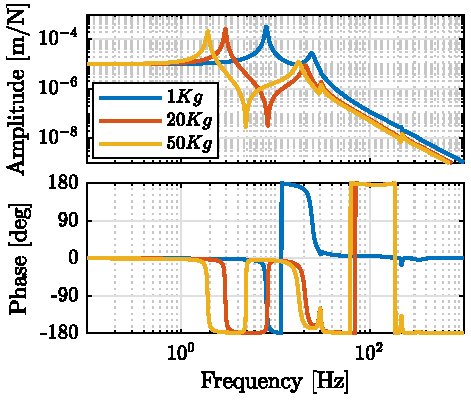
\includegraphics[scale=1]{./figs/G_x_mass.pdf}
\caption{\label{fig:G_x_mass}
Transfer function from a force applied by the NASS in the \(x\) direction to the sample displacement with respect to the granite in the \(x\) direction. This is shown for 3 values of sample mass.}
\end{figure}

As the measurement and the force applied by the NASS are in 6DoF, \(G\) is a 6 by 6 transfer function.
Figure \ref{fig:G_x_mass} represents the bode diagram of the first element of \(G\) for 3 values of the sample mass.
It shows that the sample mass has an important impact on the dynamic of the system and it confirms that we will have to be very cautious about the robustness of the controlled system.

\subsection{Control Synthesis}
\label{sec:org253eb42}
In order to control such a system, we choose to start with a simple centralized feedback control as shown Fig. \ref{fig:general_conf_K}.
The controller takes the signal of the metrology system in 6DoF and generates the forces applied by the NASS in 6DoF. It has therefore 6 inputs and 6 outputs and contains 36 elements.
We first choose to only have diagonal elements in the controller has a decoupling compensator has been used.
Tanks to that, each diagonal element can be tuned separately.

\begin{figure}[htbp]
\centering
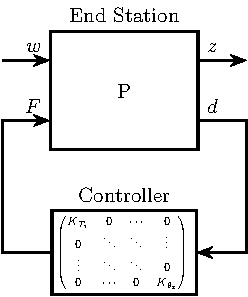
\includegraphics[scale=1]{./figs/general_conf_K.pdf}
\caption{\label{fig:general_conf_K}
General control configuration applied to the end station. \(P\) represents the model developed of the end station. \(w\) represents the exogenous inputs such has ground motion and sensor noise, \(d\) the 6DoF measurement, \(F\) the 6DoF forces applied by the NASS and \(z\) the exogenous output that we want to minimize.}
\end{figure}

A typical loop gain obtained for the \(x\) direction is shown Fig. \ref{fig:loopgain}. An integral action is added at low frequency to have no static error, and a lead is added near the crossover frequency to add some phase margin. A pole is further added in high frequency to reduce the effect of noise (not shown).

\begin{figure}[htbp]
\centering
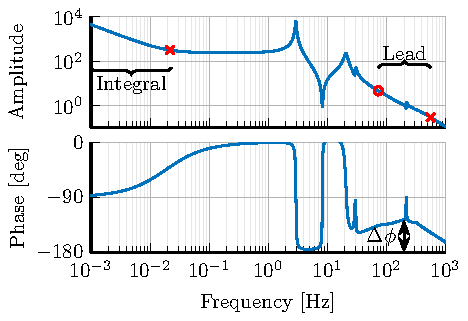
\includegraphics[scale=1]{./figs/loopgain.pdf}
\caption{\label{fig:loopgain}
Bode plot of the loop gain for the control in \(x\) direction. The red circles and the red crosses represent respectively the zeros and poles of the controller. \(\Delta\phi\) represents the phase margin.}
\end{figure}

\subsection{Tomography Experiment}
\label{sec:org05ae606}
In order to test the performances obtained with the current controlled system, a simulation of a tomography experiment is conducted.
The rotation speed of the spindle is set to \(\dot{\theta_z} = 30rpm\), the mass of the sample is chosen to be \(M=\SI{20}{\kilo\gram}\), and ground motion is taken into account.

The result is shown Fig. \ref{fig:exp_w_wo_nass_xy}. The blue and the red curves represent the \(x-y\) motion of the sample for the positioning system respectively without the NASS (corresponding to the Fig. \ref{fig:schematic_sys_without_nass}) and with the NASS (corresponding to the Fig. \ref{fig:system_control}).

The residual motion of the sample when using the NASS is less than \(\SI{50}{\nano\metre}\) in the \(xyz\) directions.

\begin{figure}[htbp]
\centering
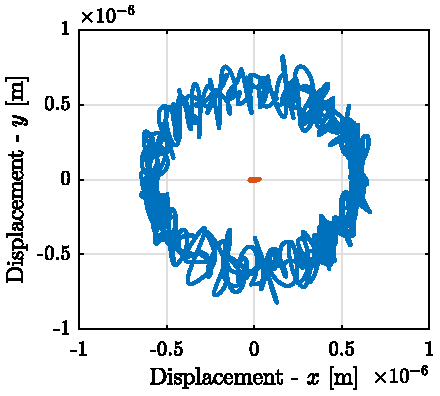
\includegraphics[scale=1]{./figs/exp_w_wo_nass_xy.pdf}
\caption{\label{fig:exp_w_wo_nass_xy}
Positioning error of the sample in the \(x\) and \(y\) direction during the simulation of a tomography experiment. The blue curve correspond with the ID31 without the NASS and the red curve with the NASS added. The sample used has a mass \(M=\SI{20}{\kilo\gram}\) and the rotational speed is \(\dot{\theta_z} = \SI{30}{rpm}\).}
\end{figure}

\section{CONCLUSION}
\label{sec:org99d6087}
A high precision and versatile positioning platform has been presented.
In order to obtain nanometer precision, a Stewart platform based stabilization system (the NASS) is proposed.
A 3D finite mass model has been developed to test such stabilization system. It has been showed that even with a simple control architecture, the parasitic motions of the sample can be reduced down to \(\SI{50}{\nano\metre}\).

These type of stabilization platform associated with a precise 6 DoF metrology system could be used for many other positioning systems.

To further improve the performance of the system, many control architecture could be developed such as a hybrid feedback-feedforward control or HAC-LAC feedback control. Moreover, to address the robustness issue, control techniques such as \(\mathcal{H}_\infty\) loop-shaping and \(\mu\)-synthesis would be of great help.

\section{ACKNOWLEDGMENTS}
\label{sec:orgb52f978}
This research was made possible by a grant from the ESRF.
We thank the following people for their support, without whose help this work would never have been possible: V. Honkimaki, A. Jublan, L. Ducotte, C. Carole, M. Brendike and M. Lessourd and the whole team of the Precision Mechatronic Laboratory.

\printbibliography
\end{document}